\documentclass{school-22.211-notes}
\date{February  8, 2012}

\begin{document}
\maketitle

\lecture{Introduction}
\topic{Course Objectives}
\begin{itemize}
  \item Continuous energy transport, reduction to multi-group diffusion group;
  \item Resonance absorption and spatial self-shielding models;
  \item Calculation of neutron spectra;
  \item Determination of few-group diffusion constants;
  \item Elementary reactor transient analysis.
\end{itemize}

\topic{Sample Exercises}
\uline{Example 1: Estimate the Mean Free Path of a Fission Neutron in an LWR} 
\begin{figure}[ht]
  \centering
  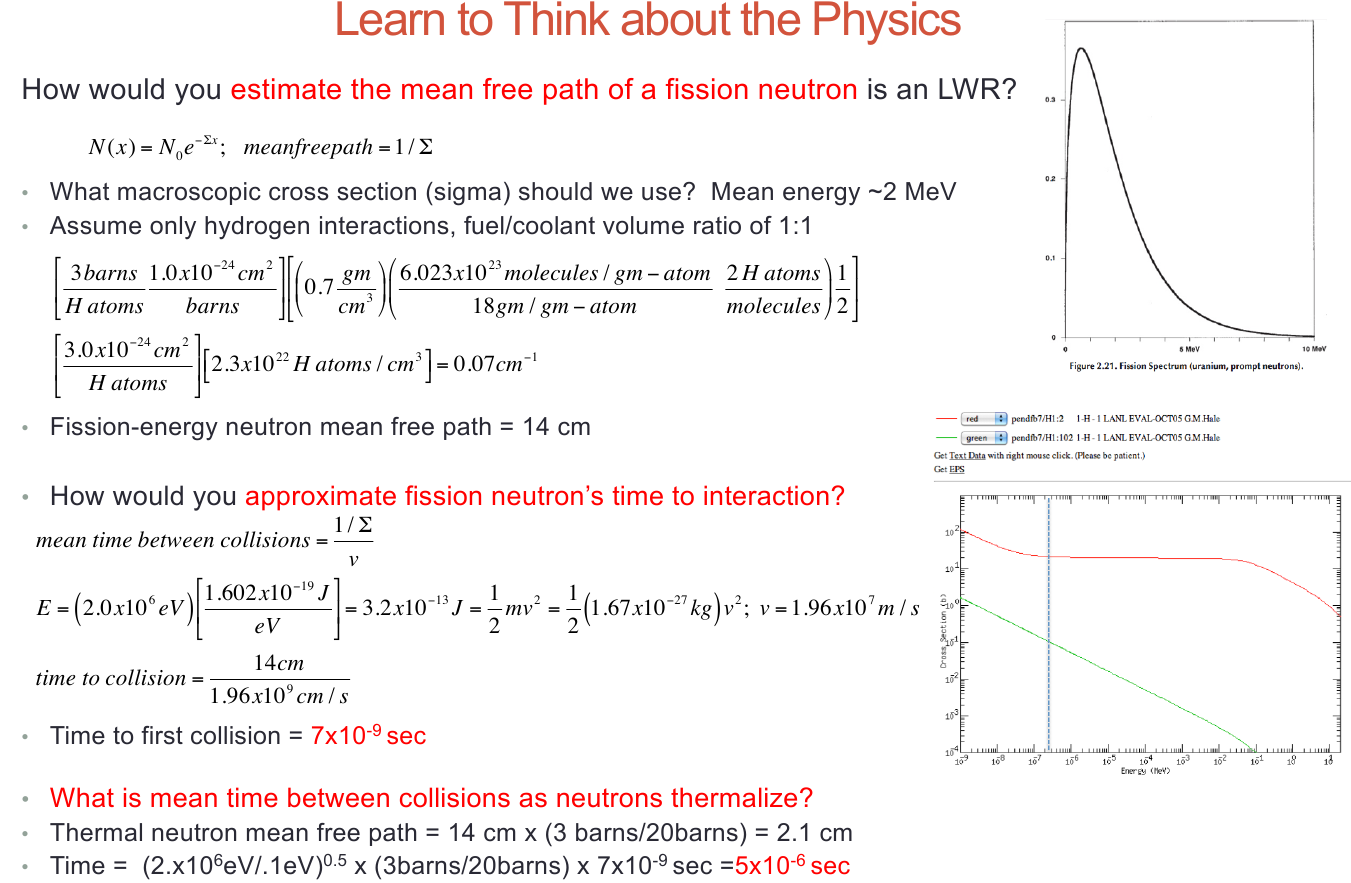
\includegraphics[width=4.5in]{images/lec1-example1.png}
\end{figure}

\uline{Example 2: Estimate Prompt Neutron Lifetime}
\begin{figure}[ht]
  \centering
  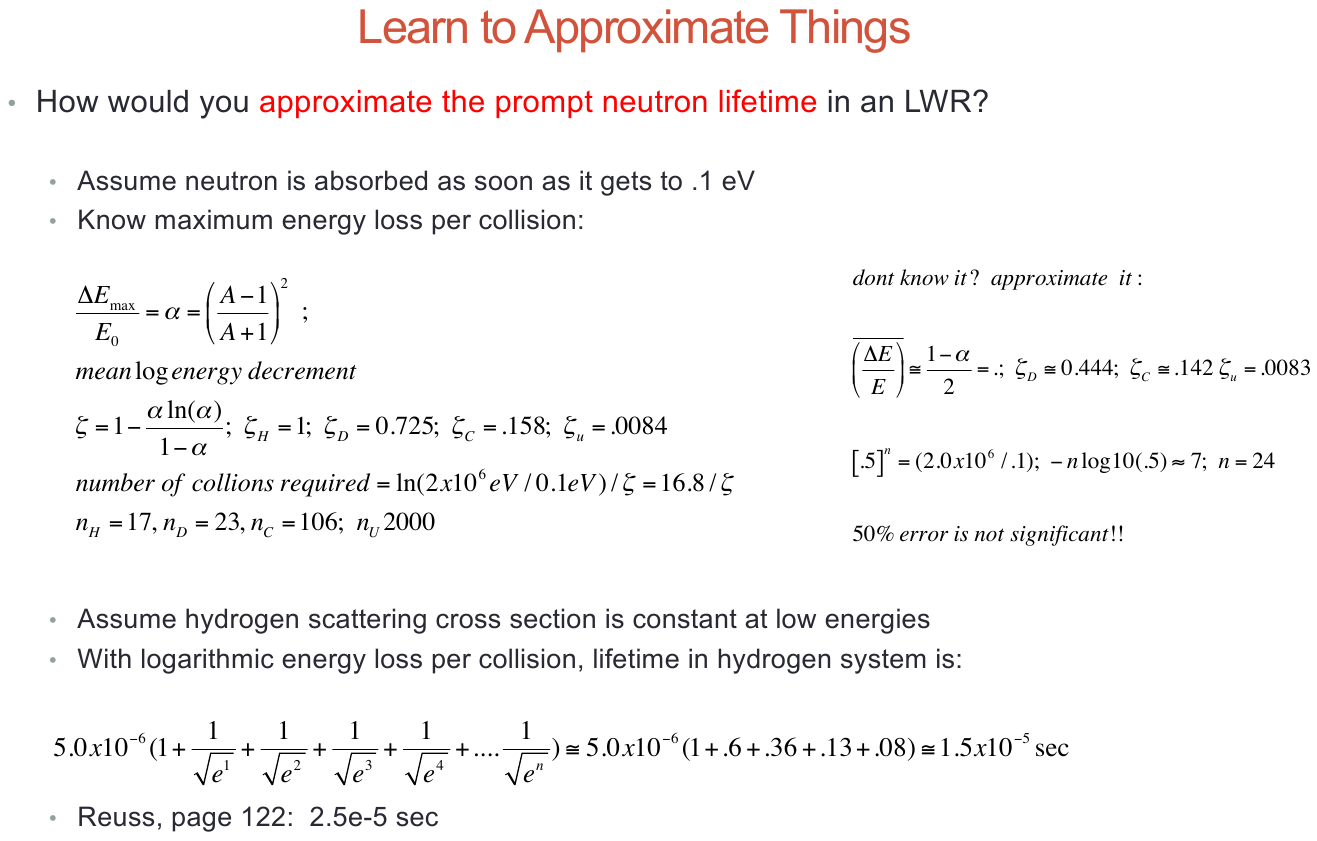
\includegraphics[width=4.5in]{images/lec1-example2.png}
\end{figure}

\uline{Example 3: Estimate Fast \& Thermal Fluxes in an LWR}
\begin{figure}[ht]
  \centering
  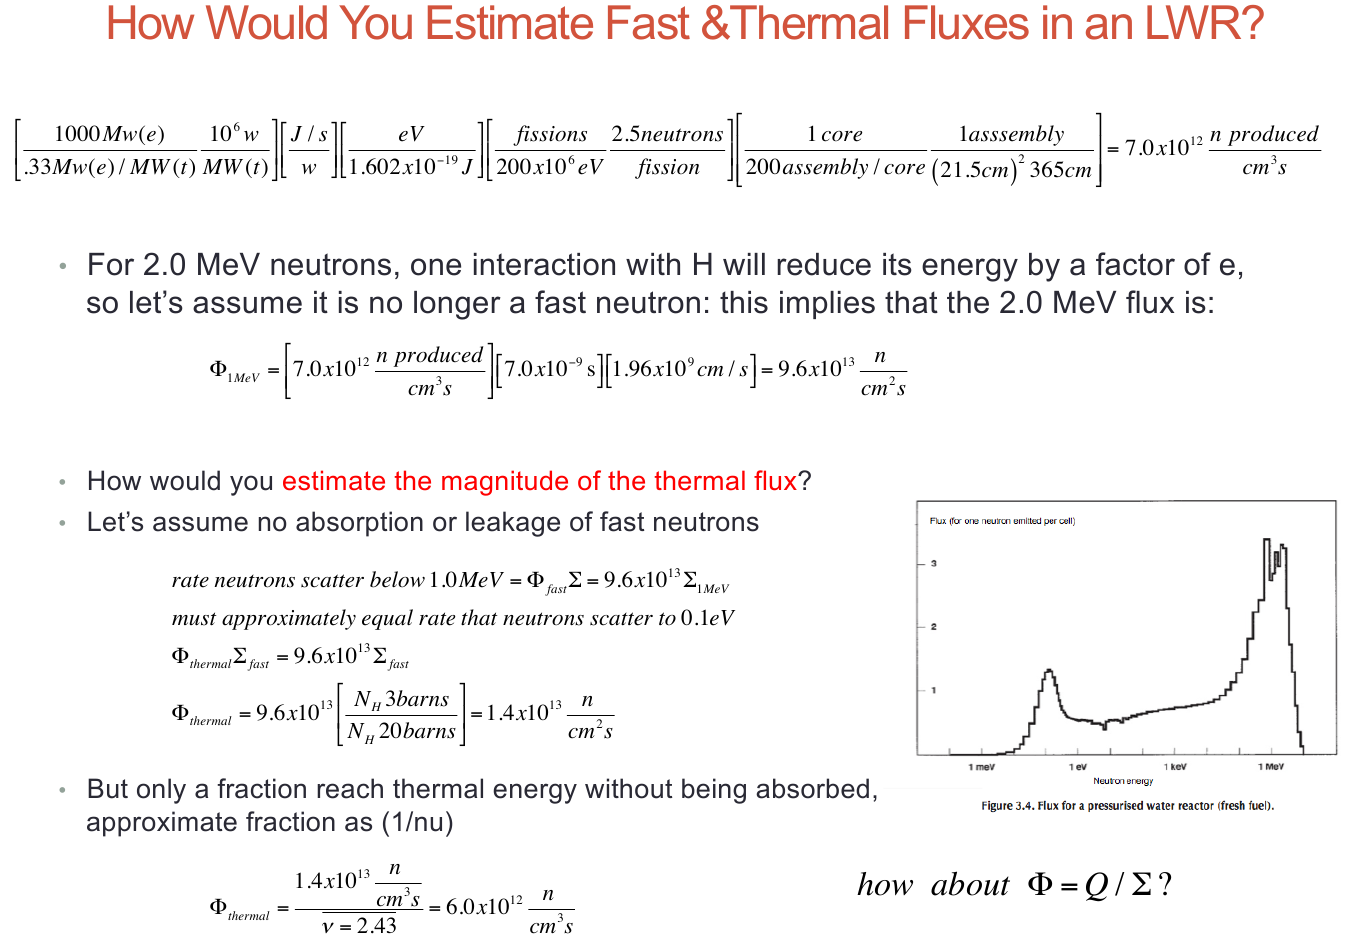
\includegraphics[width=4.5in]{images/lec1-example3.png}
\end{figure}

\topic{Summary: Reuss Ch 1 (FIXME)}

\topic{Summary: Reuss Ch 2 (FIXME)}

\topic{Summary: Reuss Ch 3 (FIXME)}

\end{document}
